\section{Constraints on Fold
Features}\label{constraints-on-fold-features}

Constraints are central to the implementation of Foldlings' algorithms,
and the pi. As an educational tool, one of the primary benefits of our
software might be the development of an intuitive understanding of the
limits of paper.

\subsection{Geometric Constraints}\label{geometric-constraints}

Several geometric constraints drive Foldling's algorithms. These
constraints are the core reason for the difficulty of creating designs
manually; a key advantage of our system is that these constraints are
resolved automatically.

\subsubsection{Box Fold}\label{box-fold}

\begin{figure}[htbp]
\centering
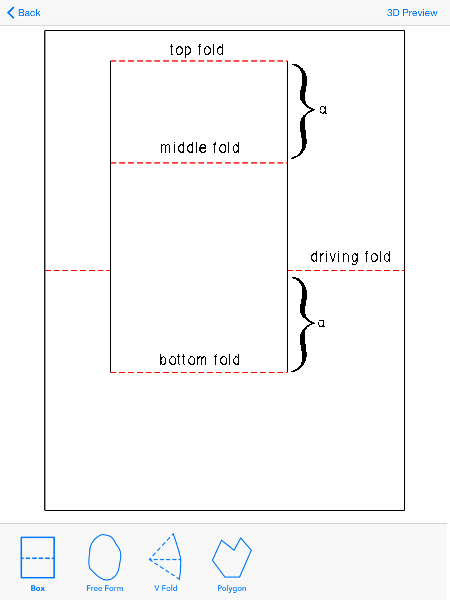
\includegraphics{figures/45_Tech_Constraints/boxfoldConstraints.pdf}
\caption{Geometric constraints for freeform features}
\end{figure}

A box fold is constrained by a relationship between its folds. Given a
top fold and bottom fold at fixed height, with a driving fold with a
height between the other two folds, the top fold must be

This 90-degree angle constraint applies equally to freeform and polygon
features (at least, those that span a fold). Holes are not bound by this
constraint, because they do not have a driving fold.

\subsubsection{Freeform}\label{freeform}

\begin{figure}[htbp]
\centering
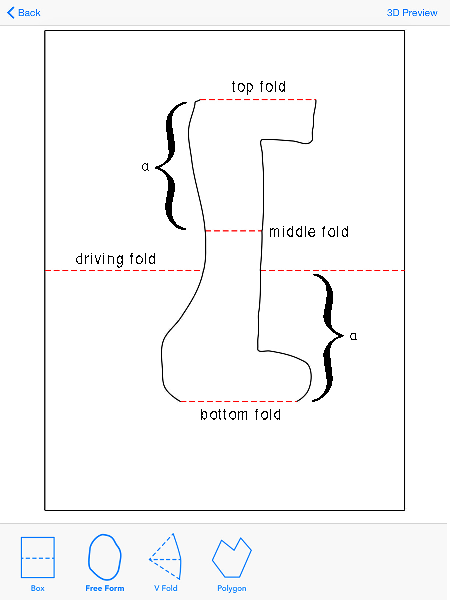
\includegraphics{figures/45_Tech_Constraints/freeformConstraints.pdf}
\caption{Geometric constraints for freeform features}
\end{figure}

A freeform shape is also constrained by. After performing truncation
\footnote{described \textbf{\textgreater{}\textgreater{}TODO: CITE}} to
place the top and bottom folds of the freeform shape, we apply the
ninety-degree constraint to place the middle fold in the feature.

\subsubsection{Polygon}\label{polygon}

\begin{figure}[htbp]
\centering
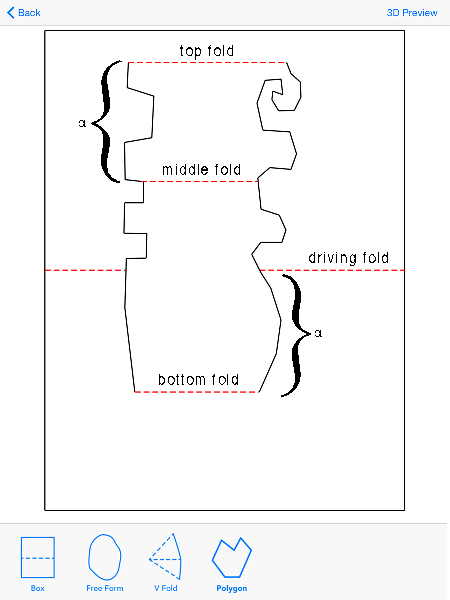
\includegraphics{figures/45_Tech_Constraints/polygonConstraints.pdf}
\caption{Geometric constraints for polygon features}
\end{figure}

The same constraints that apply to freeform shape apply to polygons.
Although the edges are constructed differently, polygons are essentially
a subset of freeform shapes, composed only of straight lines.

\subsubsection{V-Fold}\label{v-fold}

\begin{figure}[htbp]
\centering
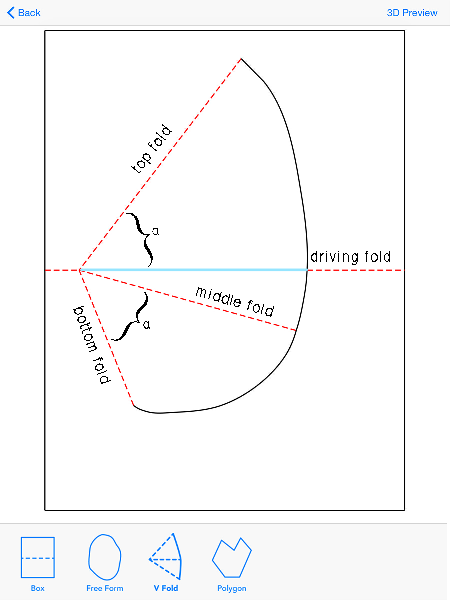
\includegraphics{figures/45_Tech_Constraints/vfoldConstraints.pdf}
\caption{Geometric constraints for freeform features}
\end{figure}

Although a v-fold also folds from zero to 180 degrees with the card, its
planes moves at non-orthogonal angles. The constraint of folds in a
v-fold feature is therefore based on angle rather than height.

The simplest case of v-folds --- and the one most popularly constructed
by our user testers using manual methods --- is a symmetric v-fold. In
this case, the top and bottom angles of the fold are equal. The shape
approximates an isosceles triangle.

In the more complex case, the angles between the two diagonal folds and
the driving fold differ.\\\textbf{\textgreater{}\textgreater{}TODO: CITE
GLASSNER}

\subsection{Physical Constraints}\label{physical-constraints}

In addition, the physicality of paper place constraints on where cuts
and folds can be placed. Depending on the manufacture method, there is
some minimum line length that can be cut or folded, and some minimum
distance folds and cuts must be apart. These depends on a wide number of
variables ranging from paper thickness to manufacture method (for
example, laser cutters have a higher tolerance for closely-drawn lines
). Even within a specific technology, there is also a wide variation in
cutting precision.

\begin{figure}[htbp]
\centering
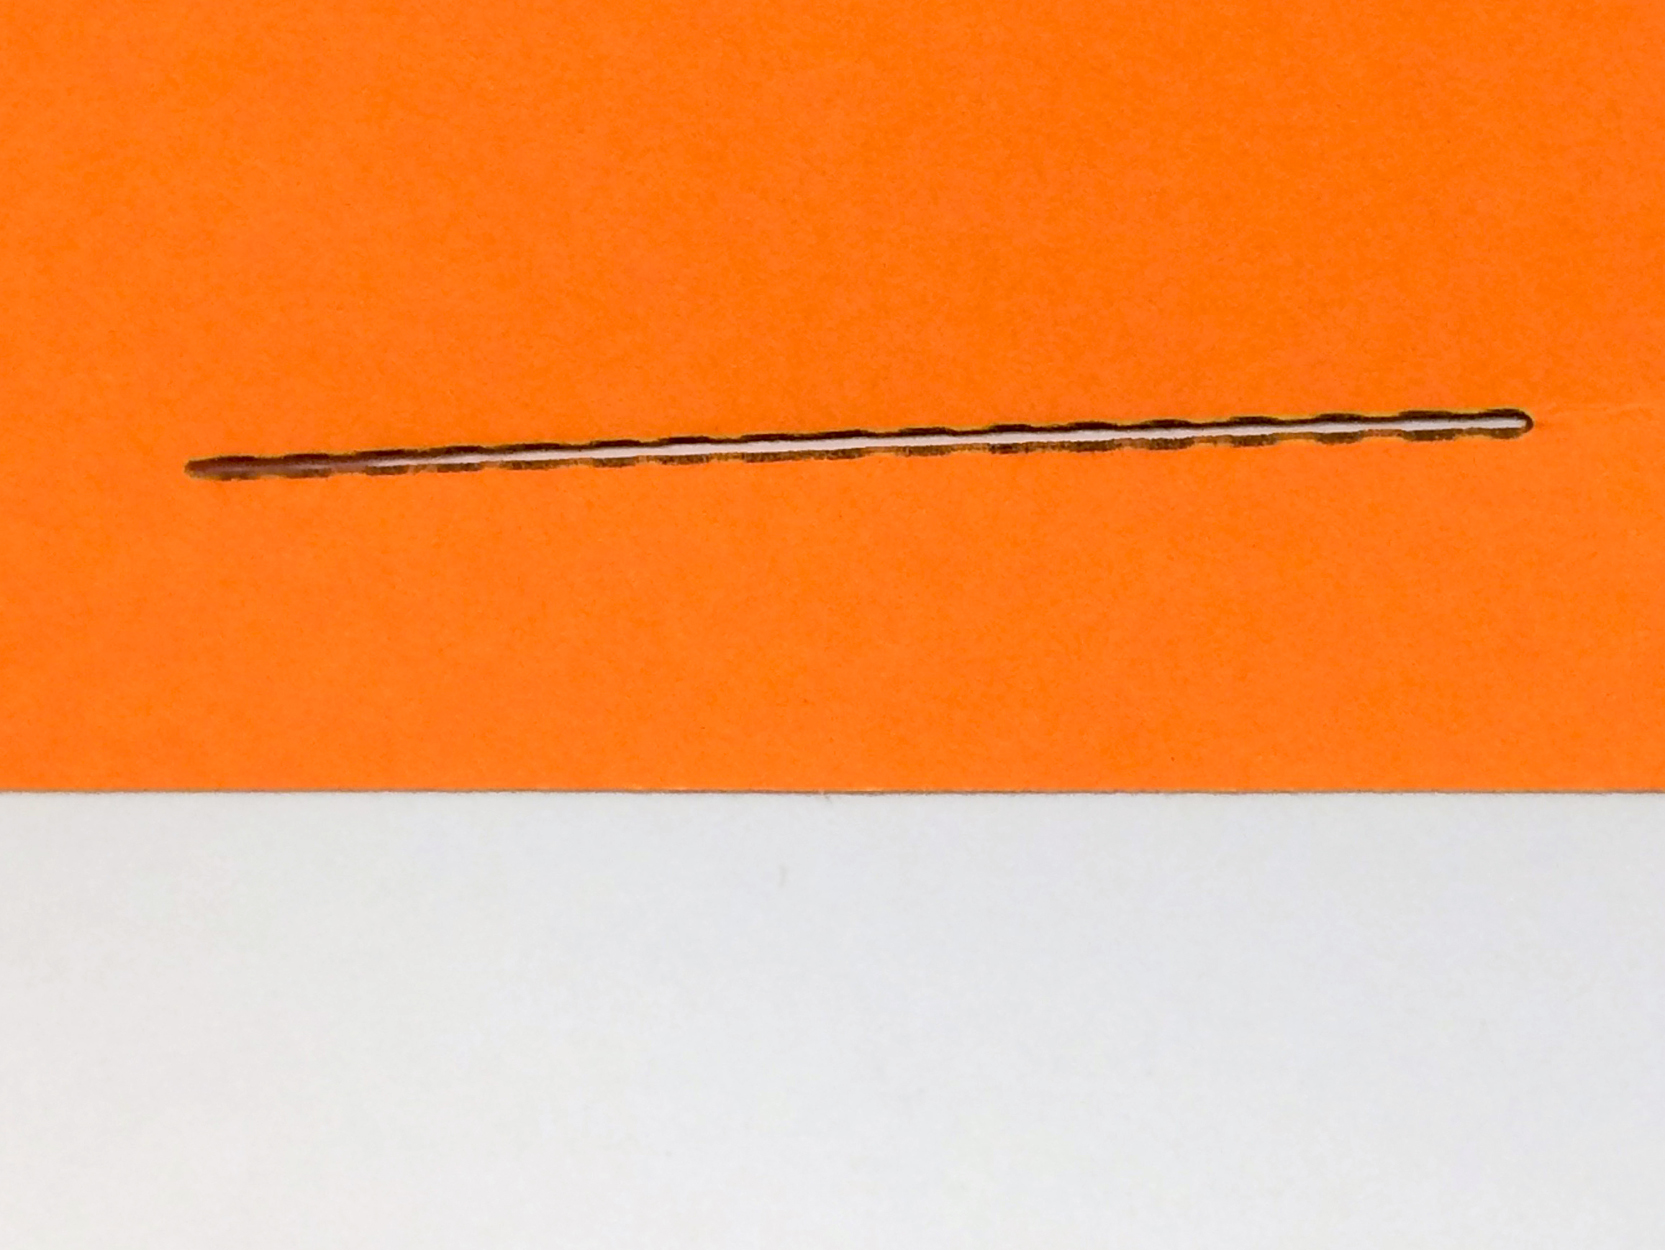
\includegraphics{figures/45_Tech_Constraints/tooclosecuts.jpg}
\caption{One constraint}
\end{figure}

In our software, we take this into account through the minimum edge
length. In addition, we . We currently

Physical. Obvious . Minimum edge length. This depends on the laser
cutter

\textbf{\textgreater{}\textgreater{}TODO: Figure showing problem}
